\chapter{Spring Data JPA}

\fcolorbox{black}[HTML]{E9F0E9}{\parbox{\textwidth}{%
\noindent \textbf{Learning goals}\\
The junior-colleague
\begin{enumerate}[nolistsep]
\item can describe the concept of ORM.
\item can explain what JPA is, and what it’s not.
\item can denominate different JPA providers.
\item can describe what a persistence unit is.
\item can explain the fundamental interfaces of JPA.
\item can explain what the persistence context is.
\item can implement entity classes.
\item can describe the entity objects’ lifecycle.
\item can implement different types of relationships between entity classes.
\item can implement CRUD operations.
\item can implement queries.
\item can implement named queries.
\item can explain, identify and solve the N + 1 query problem.
\end{enumerate}}}

  
\section{What is ORM?}

Object-Relational Mapping (ORM) is a technique that lets you query and manipulate data from a relational database using an object-oriented programming language.

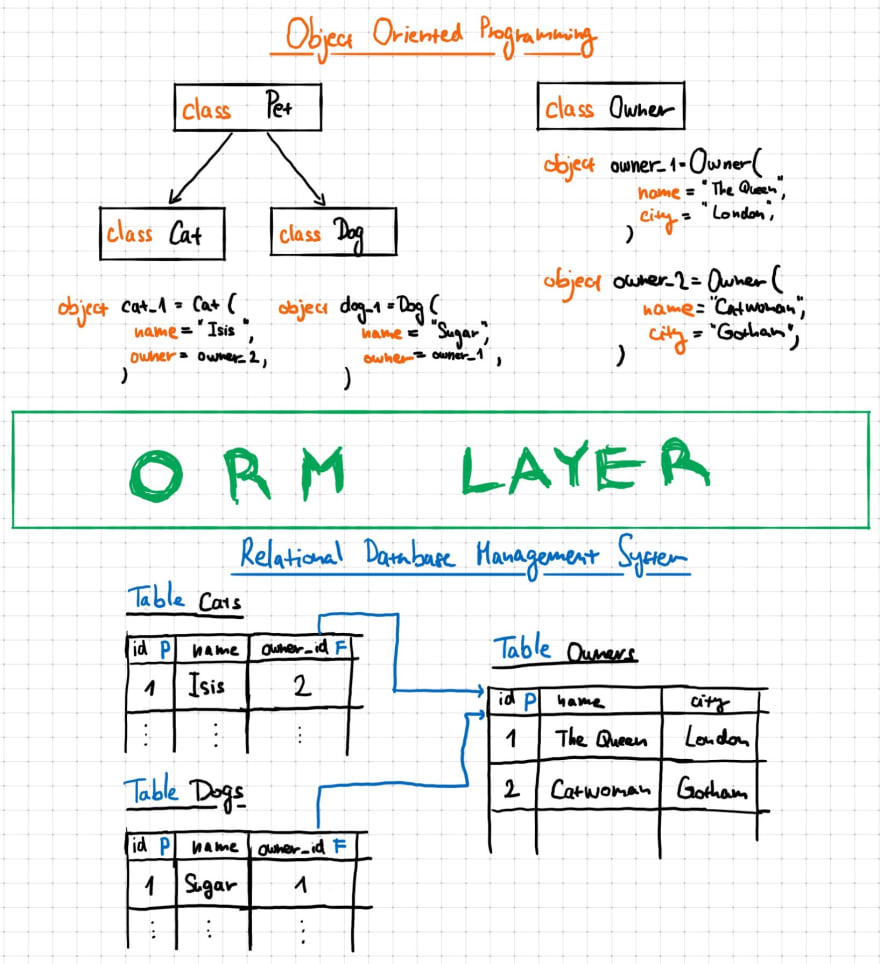
\includegraphics[width=\textwidth]{./images/chapter6/orm}


\section{What is JPA?}

The Java Persistence API (JPA; recently renamed to Jakarta Persistence API) is a specification that defines how to persist data in Java applications. JPA mainly focuses on the ORM layer and managing persistent objects.

JPA is a specification which means JPA consists of implementation guidelines for the Java ORM layer and the syntax. The specification only comes with interfaces, no actual implementation.  A reference implementation can be provided but other companies can create and distribute their own implementation of the specification.

\frame{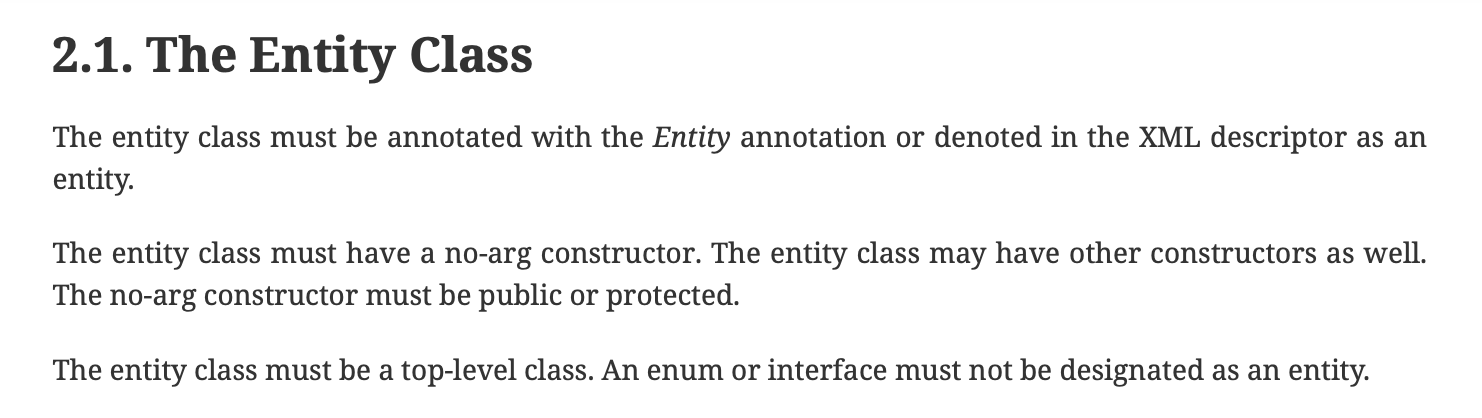
\includegraphics[width=\textwidth]{./images/chapter6/entity_class_specification}}

For our exercises and projects we will use Hibernate as the actual implementation of de JPA specification \footnote{\url{https://hibernate.org/ and https://hibernate.org/orm/}}.  

Spring Data JPA adds a layer on top of JPA. It uses all the features defined by the JPA specification, but adds no-code implementation of the repository pattern and the creation of database queries from method names.

\section{Datasource}

In Spring Boot a DataSource-object is the preferred means of getting a connection to a database.
The interface jakarta.sql.DataSource is implemented by the database driver vendor. 

The datasource can be specified in the application.properties file.

\begin{lstlisting}
spring.datasource.url=jdbc:postgresql://localhost:5432/recipes
spring.datasource.username=postgres
spring.datasource.password=postgres
\end{lstlisting}

Alternatively, the data source configuration can be programmatically.


\section{The Entity class}

\begin{lstlisting}[frame=single,language=java]
package be.pxl.paj.domain;

import org.apache.logging.log4j.LogManager;
import org.apache.logging.log4j.Logger;

import javax.persistence.Column;
import javax.persistence.Entity;
import javax.persistence.GeneratedValue;
import javax.persistence.Id;

@Entity
public class Superhero {

	private static final Logger LOGGER = LogManager.getLogger(Superhero.class);

	@Id
	@GeneratedValue
	private long id;
	private String firstName;
	private String lastName;
	private String superheroName;
	@Column(name="notes")
	private String description;

	protected Superhero() {
		// JPA only
	}

	public Superhero(String firstName, String lastName, String superheroName) {
		LOGGER.debug("Creating a new superhero...");
		this.firstName = firstName;
		this.lastName = lastName;
		this.superheroName = superheroName;
	}

	public String getFirstName() {
		LOGGER.trace("FirstName of " + superheroName + " was revealed.");
		return firstName;
	}

	public void setFirstName(String firstName) {
		this.firstName = firstName;
	}

	public String getLastName() {
		LOGGER.fatal("LastName of " + superheroName + " was revealed.");
		return lastName;
	}

	public void setLastName(String lastName) {
		this.lastName = lastName;
	}

	public String getSuperheroName() {
		return superheroName;
	}

	public void setSuperheroName(String superheroName) {
		this.superheroName = superheroName;
	}

	public String getDescription() {
		return description;
	}

	public void setDescription(String description) {
		this.description = description;
	}

	@Override
	public String toString() {
		return "Superhero{" +
				"superheroName='" + superheroName + '\'' +
				'}';
	}
}
\end{lstlisting}

A JPA entity class is a POJO (Plain Old Java Object) class  that is annotated as having the ability to represent objects in the database.

The \textbf{@Id} annotation marks a field as a primary key field.

The \textbf{@Column} annotation is used to specify the details of the column to which a field or property will be mapped. You can use column annotation with the following most commonly used attributes:
\begin{itemize}
\item \textbf{name}: specify the name of the column.
\item \textbf{length}: specify the size of thee column, particularly for a String value.
\item \textbf{nullable}: mark the column to be NOT NULL when the database schema is generated.
\item \textbf{unique}: mark the column to contain only unique values.
\end{itemize}


\section{Entity lifecycle}


Persistence units are defined by the \textit{persistence.xml} configuration file.  Based on these properties, Hibernate connects with the underlying database.  The persistence.xml file is located in the folder \textbf{src/main/resources/META-INF}.

\begin{lstlisting}[language=xml,frame=single]
<persistence xmlns="http://xmlns.jcp.org/xml/ns/persistence"
             xmlns:xsi="http://www.w3.org/2001/XMLSchema-instance"
             version="2.2"
             xsi:schemaLocation="http://xmlns.jcp.org/xml/ns/persistence http://xmlns.jcp.org/xml/ns/persistence/persistence_2_2.xsd">
	<persistence-unit name="musicdb_pu" transaction-type="RESOURCE_LOCAL">
		<properties>
			<property name="javax.persistence.jdbc.driver"
			          value="com.mysql.cj.jdbc.Driver"/>
			<property name="javax.persistence.jdbc.url"
			          value="jdbc:mysql://localhost:3306/musicdb"/>
			<property name="javax.persistence.jdbc.user" value="user"/>
			<property name="javax.persistence.jdbc.password" value="password"/>
			<property name="hibernate.show_sql" value="true" />
			<property name="hibernate.hbm2ddl.auto" value="update"/>
		</properties>
	</persistence-unit>
</persistence>
\end{lstlisting}

The persistence unit holds all the needed information for creating an EntityManagerFactory instance.  Among this information, we have details about the data source (JDBC URL, user, password, SQL dialect, etc), the list of entities that will be managed, and other specific properties. And, of course, we have the persistence-unit transaction type, which can be RESOURCE\_LOCAL or JTA. 

The EntityManager is a core interface of JPA.  An instance of EntityManager is used to create and remove  entity instances, to find entities by their primary key,  and to query over entities.  In fact,  an instance of the EntityManager is used to interact with the persistence context. 

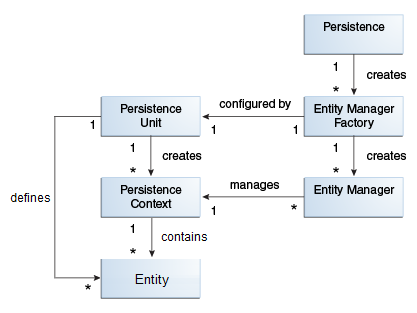
\includegraphics[width=\textwidth]{./images/chapter6/persistence}

In the examples in this chapter, the lifecycle of the EntityManager is managed by the application.
In fact, we'll manually create the EntityManager,  and we are also responsible to close the EntityManager.

The persistence context is the first-level cache where all the entities fetched from the database are managed.  Therefore, we call them managed entities.  The persistence context keeps track of any changes made to managed entities. If anything changes during a transaction, then the entity is marked as dirty. When the transaction completes, these changes are flushed into the database.
Whenever we use the EntityManager, we are actually interacting with the persistence context.

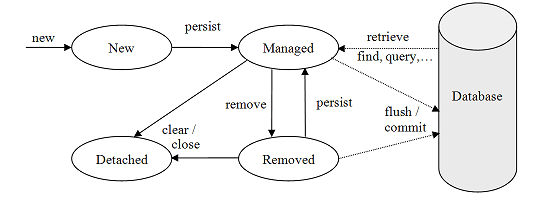
\includegraphics[width=\textwidth]{./images/chapter6/entity_states}


\section{CRUD operations}

\subsection{Storing and retrieving entities}

The EntityManager instance offers the method \textit{persist(entity)} to add totally new entities to the database.

All operations that modify the database require an active transactions. Therefore, a TransactionRequiredException is thrown if there is no active transaction when persist is called.

If the database already contains another entity of the same type with the same primary key, an EntityExistsException is thrown. The exception is thrown either by persist (if that existing entity object is currently managed by the EntityManager) or by commit.

In our Superhero example, the creation of the primary key is handled by Hibernate.
The JPA specification supports 4 different primary key generation strategies which generate the primary key values programmatically or use database features, like auto-incremented columns or sequences. The only thing you have to do is to add the @GeneratedValue annotation to your primary key attribute and choose a generation strategy. The default primary key generation strategy is GenerationType.AUTO. For most relational database systems, Hibernate will create a database sequence which generates the primary keys.  If you definitely want a database sequence you can add GenerationType.SEQUENCE. And if you decide to use auto-incremented columns you need add strategy GenerationType.IDENTITY. 
The last strategy, GenerationType.TABLE will use a specific database table for primary key generation. This last strategy will not be used in this course.

\begin{lstlisting}[frame=single, language=java]
@Id
@GeneratedValue(strategy = GenerationType.AUTO)
private Long id;
\end{lstlisting}


\begin{lstlisting}[frame=single, language=java]
package be.pxl.paj;

import be.pxl.paj.domain.Superhero;
import org.apache.logging.log4j.LogManager;
import org.apache.logging.log4j.Logger;

import javax.persistence.EntityManager;
import javax.persistence.EntityManagerFactory;
import javax.persistence.EntityTransaction;
import javax.persistence.Persistence;

public class PersistJPA {

	private static final Logger LOGGER = LogManager.getLogger(AppJPA.class);

	public static void main(String[] args) {
		EntityManagerFactory emf = Persistence.createEntityManagerFactory("musicdb_pu");
		EntityManager entityManager = emf.createEntityManager();
		Superhero superhero = new Superhero("Clark", "Kent", "Superman");
		EntityTransaction transaction = entityManager.getTransaction();
		transaction.begin();
		entityManager.persist(superhero);
		transaction.commit();
		long superHeroId = superhero.getId();
		LOGGER.info("Superhero saved with id [" + superHeroId + "]");
		entityManager.clear();

		Superhero savedSuperhero = entityManager.find(Superhero.class, superHeroId);
		LOGGER.info(savedSuperhero.getSuperheroName());
		entityManager.close();
		emf.close();
	}
}
\end{lstlisting}

This example shows how to retrieve entities by their id.  If you want to retrieve a superhero by it's superheroname, you need to write a query. There are several techniques in JPA to write queries. JPQL is one of them. Here is an example:

\begin{lstlisting}[frame=single,language=java]
package be.pxl.paj;

import be.pxl.paj.domain.Superhero;
import org.apache.logging.log4j.LogManager;
import org.apache.logging.log4j.Logger;

import javax.persistence.EntityManager;
import javax.persistence.EntityManagerFactory;
import javax.persistence.Persistence;
import javax.persistence.TypedQuery;

public class RetrieveJPA {

	private static final Logger LOGGER = LogManager.getLogger(RetrieveJPA.class);

	public static void main(String[] args) {
		EntityManagerFactory emf = Persistence.createEntityManagerFactory("musicdb_pu");
		EntityManager entityManager = emf.createEntityManager();
		TypedQuery<Superhero> query = entityManager.createQuery("SELECT s FROM Superhero s WHERE s.superheroName = :name", Superhero.class);;
		query.setParameter("name", "Superman");
		Superhero result = query.getSingleResult();

		LOGGER.info(result.getFirstName());

		entityManager.close();
		emf.close();
	}
}
\end{lstlisting}



\subsection{Updating entities}


Once an entity object is in managed state,  it can be modified and as soon as an active transaction commits, all changes are stored in the database.

\begin{lstlisting}[frame=single,language=java]
package be.pxl.paj;

import be.pxl.paj.domain.Superhero;
import org.apache.logging.log4j.LogManager;
import org.apache.logging.log4j.Logger;

import javax.persistence.EntityManager;
import javax.persistence.EntityManagerFactory;
import javax.persistence.EntityTransaction;
import javax.persistence.Persistence;

public class UpdateJPA {

	private static final Logger LOGGER = LogManager.getLogger(UpdateJPA.class);

	public static void main(String[] args) {
		EntityManagerFactory emf = Persistence.createEntityManagerFactory("musicdb_pu");
		EntityManager entityManager = emf.createEntityManager();
		Long superHeroId = 2L;
		Superhero savedSuperhero = entityManager.find(Superhero.class, superHeroId);

		EntityTransaction transaction = entityManager.getTransaction();
		transaction.begin();
		savedSuperhero.setDescription("Some description here...");
		transaction.commit();

		entityManager.close();
		emf.close();
	}
}
\end{lstlisting}

\subsection{Deleting entities}

In order to delete a managed object from the database we need to call the \textit{remove()} method during an active transaction. Once the transaction is committed, the corresponding row is physically removed from the database.


\section{Relationships}

JPA supports the same associations as you know from relational databases.

 You can use:
\begin{itemize}
\item one-to-one associations,
\item many-to-one associations and
\item many-to-many associations.
\end{itemize}
You can map each of them as a uni- or bidirectional association.


\subsection{One-to-One relationship}

In a one-to-one relationship, one record in a table is associated with one and only one record in another table.

\begin{lstlisting}[frame=single, language=java]
package be.pxl.paj.domain;

import javax.persistence.Entity;
import javax.persistence.GeneratedValue;
import javax.persistence.GenerationType;
import javax.persistence.Id;
import javax.persistence.Table;

@Entity
@Table(name = "contact_info")
public class ContactInformation {
	@Id
	@GeneratedValue(strategy = GenerationType.IDENTITY)
	private Long id;
	private String phone;
	private String email;
	private String linkedIn;

	public ContactInformation() {
	}

	public Long getId() {
		return id;
	}

	public String getPhone() {
		return phone;
	}

	public void setPhone(String phone) {
		this.phone = phone;
	}

	public String getEmail() {
		return email;
	}

	public void setEmail(String email) {
		this.email = email;
	}

	public String getLinkedIn() {
		return linkedIn;
	}

	public void setLinkedIn(String linkedIn) {
		this.linkedIn = linkedIn;
	}
}
\end{lstlisting}

The member variable with the type of the associated entity class is annotated with @OneToOne. You can customize the name of the foreign key column with a @JoinColumn annotation.

\begin{lstlisting}[frame=single, language=java]
package be.pxl.paj.domain;

import javax.persistence.CascadeType;
import javax.persistence.Column;
import javax.persistence.Entity;
import javax.persistence.GeneratedValue;
import javax.persistence.GenerationType;
import javax.persistence.Id;
import javax.persistence.OneToOne;

@Entity
public class Researcher {

	@Id
	@GeneratedValue(strategy = GenerationType.IDENTITY)
	private Long id;
	@Column(length = 40, nullable = false)
	private String name;
	@OneToOne(cascade = CascadeType.ALL)
	private ContactInformation contactInformation;

	public Long getId() {
		return id;
	}

	public String getName() {
		return name;
	}

	public void setName(String name) {
		this.name = name;
	}

	public ContactInformation getContactInformation() {
		return contactInformation;
	}

	public void setContactInformation(ContactInformation contactInformation) {
		this.contactInformation = contactInformation;
	}
}
\end{lstlisting}

The meaning of CascadeType.ALL is that the persistence context will propagate (cascade) all EntityManager operations (PERSIST, REMOVE, REFRESH, MERGE, DETACH) to the relating entities.

\subsection{Many-to-one relationship}

Next an example of a many-to-one relationship.  
Suppose there are multiple researchers working on one project, but every researcher is assigned to one project. 

Here is the entity class Project.

\begin{lstlisting}[frame=single, language=java]
package be.pxl.paj.domain;

import javax.persistence.Entity;
import javax.persistence.GeneratedValue;
import javax.persistence.GenerationType;
import javax.persistence.Id;
import java.time.LocalDate;

@Entity
public class Project {
	@Id
	@GeneratedValue(strategy = GenerationType.IDENTITY)
	private Long id;
	private String name;
	private LocalDate start;
	@Enumerated(value= EnumType.STRING)
	private ProjectPhase projectPhase;

	public Project() {
	}

	public Project(String name, LocalDate start) {
		this.name = name;
		this.start = start;
	}

	public Long getId() {
		return id;
	}

	public void setId(Long id) {
		this.id = id;
	}

	public String getName() {
		return name;
	}

	public void setName(String name) {
		this.name = name;
	}

	public LocalDate getStart() {
		return start;
	}

	public void setStart(LocalDate start) {
		this.start = start;
	}
	
	public ProjectPhase getProjectPhase() {
		return projectPhase;
	}

	public void setProjectPhase(ProjectPhase projectPhase) {
		this.projectPhase = projectPhase;
	}
}
\end{lstlisting}

\begin{lstlisting}[frame=single, language=java]
package be.pxl.paj.domain;

public enum ProjectPhase {
	INITIATING,
	PLANNING,
	EXECUTING,
	CLOSING;
}
\end{lstlisting}

The most common option to map an enum value to and from its database representation in JPA is to use the @Enumerated annotation. This way, we can instruct a JPA provider to convert an enum to its ordinal or String value.  When using the String value,  we can safely add new enum values or change our enum's order.  However, renaming an enum value will still break the database data.

To create the relation between a researcher and the project he's working on, we add a @ManyToOne relationship in the entity class Researcher.

\begin{lstlisting}[frame=single,language=java]
package be.pxl.paj.domain;

import javax.persistence.CascadeType;
import javax.persistence.Column;
import javax.persistence.Entity;
import javax.persistence.GeneratedValue;
import javax.persistence.GenerationType;
import javax.persistence.Id;
import javax.persistence.ManyToOne;
import javax.persistence.OneToOne;

@Entity
public class Researcher {

	@Id
	@GeneratedValue(strategy = GenerationType.IDENTITY)
	private Long id;
	@Column(length = 40, nullable = false)
	private String name;
	@OneToOne(cascade = CascadeType.ALL)
	private ContactInformation contactInformation;
	@ManyToOne
	private Project project;

	public Long getId() {
		return id;
	}

	public String getName() {
		return name;
	}

	public void setName(String name) {
		this.name = name;
	}

	public ContactInformation getContactInformation() {
		return contactInformation;
	}

	public void setContactInformation(ContactInformation contactInformation) {
		this.contactInformation = contactInformation;
	}

	public void setProject(Project project) {
		this.project = project;
	}

	public Project getProject() {
		return project;
	}
}
\end{lstlisting}

At the moment, it's not possible to see which researchers are working on a project. To make this possible we have to make the relationship between project and researcher bi-directional.  Researcher is defined the \textbf{owner} of the relationship. To make this association bi-directional, all we'll have to do is to define the referencing side. The inverse or the referencing side simply maps to the owning side.  The value of mappedBy is the name of the association-mapping attribute on the owning side.  The fetch type of this @OneToMany relationship is by default \textbf{lazy}. This means the researcher for a project are only retrieved from the database when the getResearchers() method is called.

\begin{lstlisting}[frame=single, language=java]
package be.pxl.paj.domain;

import javax.persistence.Entity;
import javax.persistence.GeneratedValue;
import javax.persistence.GenerationType;
import javax.persistence.Id;
import javax.persistence.OneToMany;
import java.time.LocalDate;
import java.util.ArrayList;
import java.util.List;

@Entity
public class Project {
	@Id
	@GeneratedValue(strategy = GenerationType.IDENTITY)
	private Long id;
	private String name;
	private LocalDate start;
	@OneToMany(mappedBy = "project")
	private List<Researcher> researchers = new ArrayList<>();

	public Project() {
	}

	public Project(String name) {
		this.name = name;
		this.start = LocalDate.now();
	}

	public Long getId() {
		return id;
	}

	public void setId(Long id) {
		this.id = id;
	}

	public String getName() {
		return name;
	}

	public void setName(String name) {
		this.name = name;
	}

	public LocalDate getStart() {
		return start;
	}

	public void setStart(LocalDate start) {
		this.start = start;
	}

	public List<Researcher> getResearchers() {
		return researchers;
	}

	public void addResearcher(Researcher researcher) {
		researchers.add(researcher);
	}

	public void removeResearcher(Researcher researcher) {
		researchers.remove(researcher);
	}

	@Override
	public String toString() {
		return name;
	}
}
\end{lstlisting}


\begin{oefening}
Use the programs CreateResearcherApp, CreateProjectApp and AssignResearcherApp to create some sample data.
Use the program ProjectDetailsApp to retrieve the details of a project.  Now, change the fetch type of the @OneToMany relationship to eager and retrieve the project details again. What can you tell about the queries being executed?
\end{oefening}
 
It's not a good idea to make Project owner of the relationship between Projects and Researchers.  You may end up with an inefficient database schema. More information can be found in this post: \url{https://vladmihalcea.com/the-best-way-to-map-a-onetomany-association-with-jpa-and-hibernate/}.


\subsection{Many-to-many relationship}

Actually, we want our researchers to work on multiple projects. Therefore,  we have to introduce a @ManyToMany relationship in the class Researcher. 

\begin{lstlisting}[frame=single,language=java]
package be.pxl.paj.domain;

import org.apache.logging.log4j.LogManager;
import org.apache.logging.log4j.Logger;

import javax.persistence.CascadeType;
import javax.persistence.Column;
import javax.persistence.Entity;
import javax.persistence.GeneratedValue;
import javax.persistence.GenerationType;
import javax.persistence.Id;
import javax.persistence.ManyToMany;
import javax.persistence.OneToOne;
import java.util.ArrayList;
import java.util.List;

@Entity
public class Researcher {

	private static final Logger LOGGER = LogManager.getLogger(Researcher.class);

	@Id
	@GeneratedValue(strategy = GenerationType.IDENTITY)
	private Long id;
	@Column(length = 40, nullable = false)
	private String name;
	@OneToOne(cascade = CascadeType.ALL)
	private ContactInformation contactInformation;
	@ManyToMany
	private List<Project> projects = new ArrayList<>();

	public Long getId() {
		return id;
	}

	public String getName() {
		return name;
	}

	public void setName(String name) {
		this.name = name;
	}

	public ContactInformation getContactInformation() {
		return contactInformation;
	}

	public void setContactInformation(ContactInformation contactInformation) {
		this.contactInformation = contactInformation;
	}

	public void addProject(Project project) {
		if (this.projects.contains(project)) {
				LOGGER.info("Researcher [" + name + "] already assigned to [" + project.getName() + "]");
				return;
		}
		this.projects.add(project);
		project.addResearcher(this);
	}

	public List<Project> getProjects() {
		return projects;
	}

	@Override
	public String toString() {
		return "Researcher{" +
				"id=" + id +
				", name='" + name + '\'' +
				", contactInformation=" + contactInformation +
				'}';
	}
}
\end{lstlisting}



If we want the relationship to be bi-directional, Researcher remains the owner of the relationship.  

\begin{lstlisting}[frame=single,language=java]
package be.pxl.paj.domain;

import javax.persistence.Entity;
import javax.persistence.GeneratedValue;
import javax.persistence.GenerationType;
import javax.persistence.Id;
import javax.persistence.ManyToMany;
import java.time.LocalDate;
import java.util.ArrayList;
import java.util.List;

@Entity
public class Project {
	@Id
	@GeneratedValue(strategy = GenerationType.IDENTITY)
	private Long id;
	private String name;
	private LocalDate start;
	@ManyToMany(mappedBy = "projects")
	private List<Researcher> researchers = new ArrayList<>();

	public Project() {
	}

	public Project(String name) {
		this.name = name;
		this.start = LocalDate.now();
	}

	public Long getId() {
		return id;
	}

	public void setId(Long id) {
		this.id = id;
	}

	public String getName() {
		return name;
	}

	public void setName(String name) {
		this.name = name;
	}

	public LocalDate getStart() {
		return start;
	}

	public void setStart(LocalDate start) {
		this.start = start;
	}

	public List<Researcher> getResearchers() {
		return researchers;
	}

	@Override
	public boolean equals(Object o) {
		if (this == o) {
			return true;
		}
		if (o == null || getClass() != o.getClass()) {
			return false;
		}

		Project project = (Project) o;

		return id != null ? id.equals(project.id) : project.id == null;
	}

	@Override
	public int hashCode() {
		return id != null ? id.hashCode() : 0;
	}

	public void addResearcher(Researcher researcher) {
		researchers.add(researcher);
	}

	@Override
	public String toString() {
		return name;
	}
}
\end{lstlisting}


When you execute one of the programs and look at the created database schema, you will notice that a \textbf{link table} is created for storing the many-to-many relationship.

\begin{oefening}
Implement the bi-directional many-to-many relationship between Researchers and Projects in the SampleJPAProject. Create a new program to remove a researcher from a project.  Make sure all data is managed correctly by the owner of the relationship.
\end{oefening}

\section{Implementing queries}

JPQL is the Java Persistence Query Language defined in the JPA specification. 
JPQL is developed based on SQL syntax.  Hibernate, or any other JPA implementation, has to transform the JPQL query into SQL.  Therefore,  it is a good practice to activate the logging of the SQL statements during development to check the generated SQL statements.

A complete JPQL language reference can be found on the website of OpenJPA (\url{https://openjpa.apache.org/builds/1.2.3/apache-openjpa/docs/jpa_langref.html#jpa_langref_between}).

The JPA Criteria API provides an alternative way for defining JPA queries, which is mainly useful for building dynamic queries whose exact structure is only known at runtime.  

\subsection{TypedQuery}

TypedQuery is the prefered query method if you know the type of the Query result.  Thanks to the strongly typed query result,  the developer can avoid introducing bugs in the code. 

\begin{lstlisting}[frame=single, language=java]
	public Project findByName(String name) {
		TypedQuery<Project> query = entityManager.createQuery("SELECT p FROM Project p WHERE p.name = :name", Project.class);

		query.setParameter("name", name);
		try {
			return query.getSingleResult();
		} catch (NoResultException e) {
			LOGGER.warn("No project found with name [" + name + "]");
			return null;
		}
	}
\end{lstlisting}


\subsection{NamedQuery}

We can define NamedQueries on the Entity class itself, providing a centralized, quick and easy way to read and find all entities related queries.

\begin{lstlisting}[frame=single,language=java]
package be.pxl.paj.domain;

import javax.persistence.Entity;
import javax.persistence.EnumType;
import javax.persistence.Enumerated;
import javax.persistence.GeneratedValue;
import javax.persistence.GenerationType;
import javax.persistence.Id;
import javax.persistence.ManyToMany;
import javax.persistence.NamedQuery;
import java.time.LocalDate;
import java.util.ArrayList;
import java.util.List;

@Entity
@NamedQuery(name = "ProjectsByPhaseAndMinNumberOfResearchers", query = "SELECT p FROM Project p WHERE p.projectPhase = :phase AND p.researchers.size >= :numberOfResearchers")
public class Project {
	@Id
	@GeneratedValue(strategy = GenerationType.IDENTITY)
	private Long id;
	private String name;
	private LocalDate start;
	@ManyToMany(mappedBy = "project")
	private List<Researcher> researchers = new ArrayList<>();
	@Enumerated(value= EnumType.STRING)
	private ProjectPhase projectPhase;

	public Project() {
	}

	public Project(String name) {
		this.name = name;
		this.start = LocalDate.now();
		this.projectPhase = ProjectPhase.INITIATING;
	}

	public Long getId() {
		return id;
	}

	public void setId(Long id) {
		this.id = id;
	}

	public String getName() {
		return name;
	}

	public void setName(String name) {
		this.name = name;
	}

	public LocalDate getStart() {
		return start;
	}

	public void setStart(LocalDate start) {
		this.start = start;
	}

	public List<Researcher> getResearchers() {
		return researchers;
	}

	public ProjectPhase getProjectPhase() {
		return projectPhase;
	}

	public void setProjectPhase(ProjectPhase projectPhase) {
		this.projectPhase = projectPhase;
	}

	@Override
	public boolean equals(Object o) {
		if (this == o) {
			return true;
		}
		if (o == null || getClass() != o.getClass()) {
			return false;
		}

		Project project = (Project) o;

		return id != null ? id.equals(project.id) : project.id == null;
	}

	@Override
	public int hashCode() {
		return id != null ? id.hashCode() : 0;
	}

	public void addResearcher(Researcher researcher) {
		researchers.add(researcher);
	}

	public void removeResearcher(Researcher researcher) {
		researchers.remove(researcher);
	}

	@Override
	public String toString() {
		return name;
	}
}
\end{lstlisting}


\begin{lstlisting}[frame=single,language=java]
public List<Project> findByPhaseAndMinNumberOfResearchers(ProjectPhase phase, int minNumberOfResearchers) {
		TypedQuery<Project> query = entityManager.createNamedQuery("ProjectsByPhaseAndMinNumberOfResearchers", Project.class);
		query.setParameter("phase", phase);
		query.setParameter("numberOfResearchers", minNumberOfResearchers);
		return query.getResultList();
}
\end{lstlisting}


\section{N + 1 query problem}

We have the entity-class Post and the entity-class PostComment. There is a uni-directional many-to-one relationship between PostComment and Post.  A PostComment belongs to exactly one Post however for one Post there may exist multiple PostComments.

\begin{lstlisting}[frame=single,  language=java]
package be.pxl.paj.domain.posts;

import javax.persistence.Entity;
import javax.persistence.GeneratedValue;
import javax.persistence.Id;

@Entity
public class Post {
	@Id
	@GeneratedValue
	private Long id;
	private String title;

	public Post() {
		// JPA only
	}

	public Post(String title) {
		this.title = title;
	}

	public Long getId() {
		return id;
	}

	public String getTitle() {
		return title;
	}

	public void setTitle(String title) {
		this.title = title;
	}
}
\end{lstlisting}

\begin{lstlisting}[frame=single,  language=java]
package be.pxl.paj.domain.posts;

import javax.persistence.Entity;
import javax.persistence.GeneratedValue;
import javax.persistence.Id;
import javax.persistence.ManyToOne;

@Entity
public class PostComment {
	@Id
	@GeneratedValue
	private Long id;
	@ManyToOne
	private Post post;
	private String review;

	public PostComment() {
		// JPA only
	}
	public PostComment(Post post, String review) {
		this.post = post;
		this.review = review;
	}

	public Long getId() {
		return id;
	}

	public Post getPost() {
		return post;
	}

	public void setPost(Post post) {
		this.post = post;
	}

	public String getReview() {
		return review;
	}

	public void setReview(String review) {
		this.review = review;
	}
}
\end{lstlisting}

Here's a naive implementation of a program that retrieves all the comments from the database.  For every retrieved comment, the title of the original post is displayed as well.

\begin{lstlisting}[frame=single,  language=java]
package be.pxl.paj;

import be.pxl.paj.domain.posts.Post;
import be.pxl.paj.domain.posts.PostComment;

import javax.persistence.EntityManager;
import javax.persistence.EntityManagerFactory;
import javax.persistence.Persistence;
import javax.persistence.Query;
import java.util.List;

public class PostWithComments {

	public static void main(String[] args) throws Exception {

		EntityManagerFactory emf = Persistence.createEntityManagerFactory("musicdb_pu");
		EntityManager em = emf.createEntityManager();

		List<PostComment> comments = em.createQuery("select pc from PostComment pc", PostComment.class).getResultList();
		
		for (PostComment comment : comments) {
			System.out.println(comment.getReview() + " on " + comment.getPost().getTitle());
		}

		em.close();
		emf.close();
	}

}
\end{lstlisting}

You may expect that only one query is sufficient for retrieving this data. However, if you look at the actual queries being executed, you find out there are multiple queries needed. That's not efficient! This problem is known as the N+1-problem.  There is one query for retrieving the comments and N queries for retrieving the accompanying post.

The solution is rewriting the query to retrieve the comments and posts at once. 

\begin{lstlisting}[frame=single,  language=java]
package be.pxl.paj;

import be.pxl.paj.domain.posts.Post;
import be.pxl.paj.domain.posts.PostComment;

import javax.persistence.EntityManager;
import javax.persistence.EntityManagerFactory;
import javax.persistence.Persistence;
import javax.persistence.Query;
import java.util.List;

public class PostWithComments {

	public static void main(String[] args) throws Exception {

		EntityManagerFactory emf = Persistence.createEntityManagerFactory("musicdb_pu");
		EntityManager em = emf.createEntityManager();

		List<PostComment> comments = em.createQuery("select pc from PostComment pc join fetch pc.post p", PostComment.class).getResultList();
		
		for (PostComment comment : comments) {
			System.out.println(comment.getReview() + " on " + comment.getPost().getTitle());
		}

		em.close();
		emf.close();
	}

}
\end{lstlisting}


\section{Exercises}

\begin{oefening}
Implement the entity classes Artist, Album and Song. The relationships between these classes (and the corresponding tables) are shown in the figure below.  Implement these relationships in a bi-directional way.

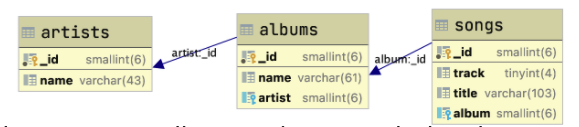
\includegraphics[width=\textwidth]{./images/chapter6/exercise-schema}

Implement the interface ArtistDao and it's implementation ArtistDaoImpl. The methods you need to implement can be found in the class diagram.

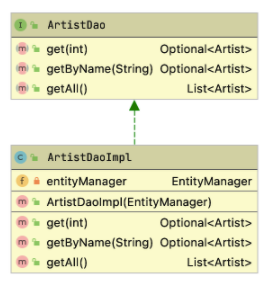
\includegraphics{./images/chapter6/exercise-dao}

Write unit tests for the class ArtistDaoImpl.

Create the program ArtistApp. A user can input the name of an artist. The program displays all the albums of the artist. For each album the songs are displayed ordered by track number.
\end{oefening}


\begin{oefening}
\textbf{Optional:} 
https://github.com/bobocode-projects/jpa-hibernate-exercises/tree/master/photo-comment-dao
\end{oefening}


\section{Spring Data JPA}

Spring Data JPA, part of the larger Spring Data family, makes it even easier to implement JPA based repositories.


\begin{lstlisting}[frame=single, language=java]
package be.pxl.superhero.repository;

import be.pxl.superhero.domain.Superhero;
import org.springframework.data.repository.JpaRepository;
import org.springframework.stereotype.Repository;

@Repository
public interface SuperheroRepository extends JpaRepository<Superhero, Long> {

	Optional<Superhero> findSuperheroBySuperheroName(String superheroName);
}
\end{lstlisting}

SuperheroRepository extends the JpaRepository interface. The type of entity and ID that it works with, Superhero and Long, are specified in the generic parameters on JpaRepository. By extending JpaRepository, SuperheroRepository inherits several methods for working with Superhero persistence, including methods for saving, deleting, and finding Superhero entities.

Spring Data JPA also lets you define other query methods by declaring their method signature. For example, CustomerRepository includes the findSuperheroBySuperheroName() method.

In a typical Java application, you might expect to write a class that implements SuperheroRepository. However, that is what makes Spring Data JPA so powerful: you don't need to write an implementation of the repository interface. Spring Data JPA creates the implementation when you run the application.

The JpaRepository interface is an extension of CrudRepository.
JpaRepository extends PagingAndSortingRepository which in turn extends CrudRepository.

Their main functions are:

\begin{itemize}
\item CrudRepository mainly provides CRUD functions.
\item PagingAndSortingRepository provides methods to do pagination and sorting records.
\item JpaRepository provides some JPA-related methods such as flushing the persistence context and deleting records in a batch.
\end{itemize}

\subsection{Unit testing a repository}

Spring Data JPA offers an annotation @DataJpaTest which makes repository testing possible with a minimum of configuration. 


\begin{lstlisting}[frame=single, language=java]
package be.pxl.superhero.repository;

import be.pxl.superhero.builder.SuperheroBuilder;
import be.pxl.superhero.domain.Superhero;
import org.junit.jupiter.api.BeforeEach;
import org.junit.jupiter.api.Test;
import org.springframework.beans.factory.annotation.Autowired;
import org.springframework.boot.test.autoconfigure.orm.jpa.DataJpaTest;

import javax.persistence.EntityManager;
import javax.persistence.PersistenceContext;
import java.util.Optional;

import static org.junit.jupiter.api.Assertions.assertEquals;
import static org.junit.jupiter.api.Assertions.assertTrue;

@DataJpaTest
public class SuperheroRepositoryTest {

	private static final String SUPERHERO_NAME = "Superman";

	@PersistenceContext
	protected EntityManager entityManager;

	@Autowired
	private SuperheroRepository superheroRepository;

	private Superhero superhero = SuperheroBuilder.aSuperhero().withFirstName("Clark").withLastName("Kent").withSuperheroName(SUPERHERO_NAME).build();

	@BeforeEach
	public void init() {
		superheroRepository.save(superhero);
		entityManager.flush();
		entityManager.clear();
	}

	@Test
	public void returnsSuperheroWithGivenSuperheroName() {
		Optional<Superhero> superheroUnderTest = superheroRepository.findSuperheroBySuperheroName(SUPERHERO_NAME);

		assertTrue(superheroUnderTest.isPresent());
		assertEquals(SUPERHERO_NAME, superheroUnderTest.get().getSuperheroName());

	}

	@Test
	public void returnsEmptyOptionalWhenNoInstituteWithGivenName() {
		Optional<Superhero> superheroUnderTest = superheroRepository.findSuperheroBySuperheroName("Robin Hood");

		assertTrue(superheroUnderTest.isEmpty());
	}
}

\end{lstlisting}





